\documentclass[sigconf, dvipsnames]{acmart}

\usepackage{xeCJK}

\usepackage{algorithm}
\usepackage{algorithmic}
\usepackage{multirow}
\usepackage{soul}
% \usepackage{balance}
 \usepackage{relsize}
 \usepackage{colortbl}
 \definecolor{paleblue}{RGB}{194,207,237}
 \definecolor{english}{rgb}{0.0, 0.5, 0.0} %wow!! http://latexcolor.com/
 \renewcommand{\labelitemi}{$\mathsmaller{\circ}$}
 \usepackage{mathtools}
\usepackage{etoolbox}
\AtBeginEnvironment{quote}{\singlespacing}

\usepackage[english]{babel}
\usepackage{blindtext}
\newcommand{\V}{\mathcal{V}}
\newcommand{\M}{\mathcal{M}}
\newcommand{\Scal}{\mathcal{S}}
\newcommand{\Pro}{\mathrm{Pr}}
\newcommand{\F}{\mathcal{F}}
\renewcommand{\floatpagefraction}{.8}%

\newcommand{\dcp}[1]{\textcolor{blue}{{\scriptsize{David:}}#1}}
\newcommand{\dcpadd}[1]{\textcolor{english}{#1}}
\newcommand{\dan}[1]{\textcolor{DarkOrchid}{{\scriptsize{Dan:}}#1}}
\newcommand{\rithvik}[1]{\textcolor{cyan}{{\scriptsize{Rithvik: }}[[#1]]}}
\newcommand{\rithvikadd}[1]{\textcolor{cyan}{#1}}
\newcommand{\mike}[1]{\textcolor{Maroon}{{\scriptsize{Mike: }}#1}}

\newcommand*{\util}{U_A}
\newcommand*{\reward}{R_A}


\renewcommand{\abstractname}{\textbf{\large {摘\quad 要}}} %更改摘要二字的样式

    \makeatletter
\def\@fnsymbol#1{\ensuremath{\ifcase#1\or \dagger\or \ddagger\or
   \mathsection\or \mathparagraph\or \|\or **\or \dagger\dagger
   \or \ddagger\ddagger \else\@ctrerr\fi}}
    \makeatother

%%
%% \BibTeX command to typeset BibTeX logo in the docs
\AtBeginDocument{%
  \providecommand\BibTeX{{%
    \normalfont B\kern-0.5em{\scshape i\kern-0.25em b}\kern-0.8em\TeX}}}

\begin{document}

\title{Uniswap V3 流动性供应策略}

\author{Michael Neuder}
\affiliation{%
\institution{Harvard University}
}
\email{michaelneuder@g.harvard.edu}

\author{Rithvik Rao}
\affiliation{%
\institution{Harvard University}
}
\email{rithvikrao@college.harvard.edu}

\author{Daniel J. Moroz}
\affiliation{%
\institution{Harvard University}
}
\email{dmoroz@g.harvard.edu}

\author{David C. Parkes}
\affiliation{%
\institution{Harvard University}
}
\email{parkes@eecs.harvard.edu}

\author{翻译:杜荣政}
\affiliation{%
\institution{Hotpot Funds}
}
\email{drz@easyman.com.cn}

\begin{abstract}
    \quad Uniswap 是加密资产领域最大的去中心化交易所。最新的Uniswap v3,允许做市商在一个或多个有限的资产价格区间内注入流动性,
    取代了v2中在所有价格区间上注入。当资产价格在价格区间内时,根据流动性所占的比例,做市商可以获得手续费收益。
    这就引出了{\em 流动性供应策略}问题:更小的价格区间意味着更聚焦的流动性,当价格维持在区间内时带来更高的收益,但同时也有更大
    的风险。我们分析了该问题,研究了3种流动性注入策略: 均匀分布(uniform), 比例分配(proportional), 以及最优策略(通过求接约束优
    化 {\em (Constrained Optimization)} 实现)。我们根据以太坊的历史价格数据给出了实验结果,结果表明,简单的流动性注入策略可以
    产生接近最优的效果,并比注入Uniswap v2流动性多赚200多倍。
\end{abstract}

\keywords{区块链, 去中心化金融, Uniswap v3, 注入流动性}

\maketitle

\section{介绍}\label{sec:intro}
\quad 去中心化金融 (DeFi) 是加密资产和区块链经济体系中一个庞大且快速增长的应用集。从2020年5月到2021年5月,尤其是2020年被称作"DeFi夏天"
的一段快速增长期,DeFi协议中的TVL(总锁定值,代表注入到协议中的所有流动性总和)增长了100倍,从8亿美元增长到800亿美元\cite{defipulse}。
DeFi的目标是用在区块链上执行的智能合约,替代传统金融中的中介机构和基础设施(典型的是以太坊)。

去中心化交易所(DEXes)允许用户之间交易不同种类的代币,而不通过一个受信中介。大多数去中心化交易所,包括Uniswap,都属于 {\em 恒等函数
做市商} (CFMMs)。作为传统交易所使用订单薄的替代,CFMMs使用{\em 自动做市商} (AMM)来决定资产价格。在 {\em Uniswap v2} 中,交易对中的
两种代币使用 {\em 流动池} 相互兑换,每个流动池由两种代币组成。交易由 {\em 储备曲线} 决定,$x y= k$,这里 $x$ 和 $y$ 分别代表流动池中
两种代币的数量, $k$ 在交易过程中保持恒定。{\em 做市商} 向流动池注入代币,供交易者交易,同时获得交易者支付的手续费。一个说明性的
储备曲线如图~\ref{fig:v2v3} (蓝色曲线)所示。交易者在用某些 $y$ 代币交易某些 $x$ 代币的过程中,资产的乘积保持恒定,例如,用 $\Delta y$ 的 $y$ 
代币,购买 $\Delta x$ 的 $x$ 代币,计算公式为 $(x-\Delta x) (y + \Delta y) = k$。

该储备曲线同时有效定义了一个以 $y$ 代币数量计价的 $x$ 代币价格,即,$p_x(x,y) = -dy/dx$ \cite{krishnamachari2021dynamic}。
在 Uniswap v2 的 $xy = k$ 曲线中,我们有 $y=k/x \implies p_x(x,y) = k/x^2$。为了方便,我们后续在对应AMM和流动池时提到的 ``价格",
都是指 $x$ 代币价格,即,$p_x(x,y)$,并且 $x$ 代币的价格波动也是相对于 $y$ 代币。

%
在Uniswap v2中,每一次交易者使用流动池交易,都会产生一个恒定的 0.3\% \cite{adams2020uniswap}手续费,由做市商获得。每一个做市商
都是在所有可能的价格区间 $(0, \infty)$ 上注入流动性,获得的手续费根据其在流动池中的流动性占比分配。\footnote{极端情况下,即,
$\lim_{x\to \infty} k/x^2 = 0$,且  $\lim_{x\to 0^+} k/x^2 = \infty$,说明该曲线支持的价格区间是 $(0,\infty)$。}

2021年5月3日,Uniswap新的协议版本,被称作 {\em Uniswap v3} \cite{adams2021uniswap},在以太坊主链发布。Uniswap v3 相对于 Uniswap v2
最大的变化是增加了 \textit{聚焦流动性} \cite{adams2021uniswap}。3周内,新协议吸引了超过12亿美元的TVL,以及日平均16亿美元的交易额 
\cite{univ3_analytics}。

%
在Uniswap v3,做市商可以向任意数量的价格区间注入流动性,称作 {\em 头寸}。价格区间在 $[p_a,p_b]$ 的头寸,当价格处于该区间内时可以
获得手续费。如果多个做市商在包含当前价格的区间内注入了流动性,获得的手续费由他们在该价格的流动性占比决定。

%
图~\ref{fig:v2v3} (红色曲线) 演示了 Uniswap v2 的恒定乘积曲线,如何被平移到与坐标轴相交,相交处的$a$ 和 $b$ 分别是该头寸
的价格区间上限和下限。这条平移后的曲线 \cite{adams2021uniswap} 由下列公式给出
\begin{align}\label{eq:v3_curve}
    \left(x + \sqrt{k / p_b} \right) \left(y +\sqrt{k p_a}\right) = k,
\end{align}
交点 $a$ 和 $b$,可以通过设 $x$ 或 $y$ 等于0得到。
%
\begin{figure}
    \centering
    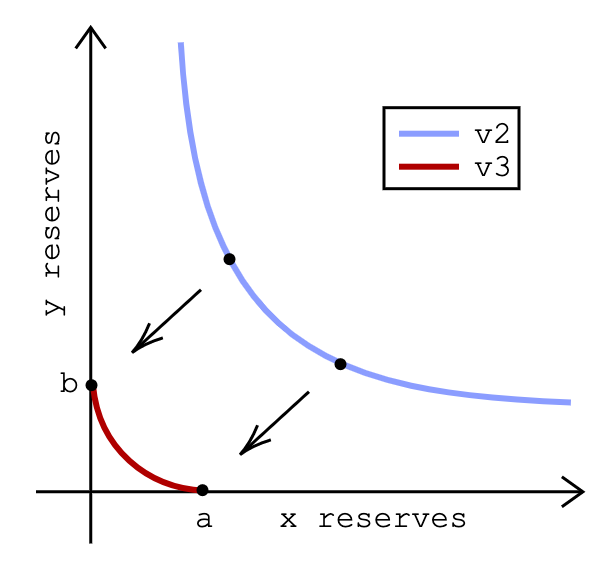
\includegraphics[width=0.5\linewidth]{img/v2v3.png}
    \caption{Uniswap v2 和 v3的储备曲线。在v3中,在价格区间 $[p_a,p_b]$ 注入聚焦流动性,导致平移 Uniswap v2 $xy=k$ 曲线与坐标轴在 $a$ 和 $b$ 处相交。交点可通过在v3储备曲线中设 $x$ 和 $y$ 等于0得到 (参见公式~\ref{eq:v3_curve}).
    \label{fig:v2v3}}
\end{figure}

通过这种方式,Uniswap v3支持流动性分配方面的多种策略。每个做市商都需要进行权衡,是选择涵盖更多可能价格的宽头寸,但赚取的手续费低于窄头寸,
还是选择更聚焦的头寸,但同时伴随更大的风险。

%dcp edit The liquidity allocation can also be adjusted based on how much risk or variance of rewards that the provider desires.
另外,重置流动性会产生费用,因为流动性分配是区块链上的交易,需要支付矿工费。这部分费用必须纳入做市商策略考虑之中。

本文的贡献如下:
\begin{enumerate}
    \item[(1)] 正式提出流动性注入策略问题,正式推出一套我们称作 ``重置流动性策略''的流动性注入策略,
    \item[(2)] 为做市商提供3种重置流动性策略, 我们分别称作 \textit{均匀分布 (uniform)}, \textit{比例分配 (proportional)},和 \textit{最优策略 (optimal)},
    \item[(3)] 分析计算重置流动性策略的预期效果, 
    \item[(4)] 基于以太坊历史价格数据创建价格变化统计信息,求解最优重置流动性策略,
    \item[(5)] 证明比例分配对于有风险偏好的做市商是最优的,而均匀分布对于风险厌恶的做市商是最优的,以及
    \item[(6)] 对最优重置流动性策略进行回归测试,证明在适当条件下,做市商的投资回报率比Uniswap v2高200倍。
\end{enumerate}

% \begin{itemize}
%     \item Rise of DeFi
%     \item Role and history of UniSwap, perhaps pointing to an illustration of v2 vs v3 (the same illustration can be pointed to from the v3 section)
%     \item v3 proposal and timing
%     \item Contribution of this paper
% \end{itemize}

\subsection{相关工作}
\quad Uniswap v1 协议参见 \citet{uniswapv1white} ,后续的 v2 参见 \cite{adams2020uniswap} 定义,最近修改的 v3 参见 \citet{adams2021uniswap}。
%

现在有越来越多针对 Uniswap v2 流动性激励的研究。
\citet{angeris2019analysis} 提供了对 Uniswap 的分析,并分析了更广泛的恒定乘积自动做市商,论证了该市场密切跟踪外部参考市场的状态。
\citet{angeris2020improved} 扩展了该研究,论证了更一般意义的恒定函数做市商,能够激励市场参与者提供外部参考市场的资产价格,论证了其作为价格预言机的价值。

\citet{evans2020liquidity} 论证了对 {\em 几何平均价做市商} (G3Ms) 而言,被动注入流动性可以被用于复制金融衍生品的收益,和更积极的交易策略。
\citet{tassy2020growth} 和 \citet{uniswapsfinancialalchemy} 分析了对价格的几何布朗运动过程中,恒定函数做市商的财富增长状况。
\citet{evans2021optimal} 将该研究扩展到更一般的做市商目标和扩散过程。

\citet{aoyagi2020lazy} 研究了恒定乘积市场的流动性均衡注入问题,表明在 Uniswap v2 环境中,策略化的做市商在与竞争对手的流动性注入参数对比时,可能具有非单调的最佳响应方式。
\citet{angeris2020does} 将该研究扩展到任何恒定函数做市商市场,并根据定义该恒定函数的曲线,计算了做市商的获利界限。

上述工作针对 Uniswap v2 和一般意义的恒定函数做市商市场,但没有针对 Uniswap v3。\citet{charmalphavault} 的一篇博客描述了一种 v3 的 ``被动重置'' 策略,
其目标在于保持做市商两种代币价值的 50-50 分配比率。我们的工作为 Uniswap v3 提供了一种更一般意义的流动性注入策略,引入马尔可夫模型来评估不同策略的预期效果。
据我们所知,这是首次正式研究 Uniswap v3 中的流动性注入策略。

\subsection{概述}
\quad 章~\ref{sec:uniswap} 介绍 Uniswap v3 协议,以及流动性注入策略的原则。我们主要聚焦于一类我们称之为 ``$\tau$-重置'' 的策略。
章~\ref{sec:markov} 阐述用马尔可夫模型分析该类策略的预期效果。
章~\ref{sec:strats} 阐述了3种流动性注入策略,包括最优 $\tau$-重置 策略。
章~\ref{sec:results} 根据以太坊历史价格数据给出实验结果。
章~\ref{sec:conclusion} 提出未来研究的开放性问题并得出结论。

\section{Uniswap v3}\label{sec:uniswap}

\quad Uniswap v3 给自动做市商市场引入了 \textit{聚焦流动性} 概念。与在所有价格区间 $(0,\infty)$ 提供流动性不同,做市商可以指定1个或多个特定的资产价格区间注入流动性。
当价格位于他设定的价格区间时,做市商可以获得手续费收益。另外,如果多个做市商在同一价格注入了流动性,他们所获得的手续费收益,根据他们在该价格处拥有总流动性的比例确定。

%A rational provider will seek to maximize their expected utility from investment in the reserve pool. 

通过选择更聚焦的价格区间,当价格位于价格区间内时,做市商可以获得更多收益,同时也会加大收益的变化幅度。
为了将其建模,我们设定了一组离散的价格区间,模拟做市商选择在每个区间注入多少流动性,何时重置流动性,以及采用何种策略来获得最大化的预期效果。

%
\begin{definition}[价格区间]
我们定义了一组 {\em 价格区间} $B = \{b_1, b_2, \ldots, b_c, \ldots\}$, 每个区间 $b_i$ 对应价格 $[l_i,r_i)$, 价格区间属于  $[0, \infty)$, 
其中 $l_1=0$ 且 对于所有 $i\in \{ 1, 2, \dots \}$ 而言 $r_i=l_{i+1}$,即每个区间的价格上限是后一个区间的价格下限。 
价格区间 $b_i$ 对应价格 $[l_i,r_i)$. $b_c$ 表示包含资产 {\em 当前价格} 的区间。
\end{definition}

在本文的后续部分,我们所指某种资产的价格都是以流动池中另一种代币为单位。例如,\texttt{USDC/ETH} 流动池,我们以 USDC 稳定币为单位来衡量 ETH 的价格波动。
当时间位于 $t=n$,用 $P_n$ 表示波动资产的当前价格。 
%
一种 {\em 流动性注入策略},代表在时间 $t=n$ 处采取何种方式在每个区间分配做市商的流动性。
%
我们做了如下假设:
%
\begin{enumerate}
    \item \textit{价格分布是恒定的---} 我们假设相对于当前价格而言,头寸的价格变化百分比,在任何时间都是恒定的。
    我们用以太坊10分钟历史价格数据进行了实证验证,我们发现以下情形的概率分布相关系数为 $r^2=0.98$ 
    (i) ETH 价格高于300美元,相对以太坊价格低于300美元
    (ii) 以太坊从 2018/4 - 2019/4 的价格,相对以太坊从 2019/4 - 2020/4 的价格。
    %
    \item \textit{重置流动性时费用是固定的---} 我们假设重置流动性的费用,也就是重置所需的 gas 费是固定的 (固定为 1美元),或者其他固定值。
    %dcp edit \footnote{Of course, this choice allows our framework to accommodate, in effect, any constant reallocation cost $c$.} 
    For example if the liquidity provider allocates $\ell=100$ units of liquidity, 
    this is interpreted as 100 times the cost of reallocating  liquidity.
    %footnote{The cost of reallocating liquidity comes from the gas fee of including a transaction a block.}
    %
    \item \textit{周期性更新---} 我们假设做市商注入的流动性是周期性更新,并且重置之后立即生效。另外,我们设定足够长的周期 (至少10分钟),并且不考虑网络传输延迟因素,那不是本项研究的重点。
    %
    \item \textit{单一策略做市商---} 我们假设了一个采用单一策略的做市商,并隐含地将其他做市商建模为在所有价格区间注入流动性,也即是采用 Uniswap v2 的流动性注入方式。
    %dcp edit This allows us to study the optimal allocation for a single-agent. In Section~\ref{sec:future}, we discuss the future work of multi-agent strategic liquidity provision, which is a natural extension to this work.
\end{enumerate}

% In regard to~(2), in reality the fee would depend on the number of bins that liquidity is being allocated to, because bin represents a different position and thus is . Since we consider situations where the provider is providing liquidity on the order of 100x the cost of moving the liquidity, we choose not to model this detail. 

\subsection{流动性注入策略}\label{sec:lpstrat}

\quad 在阐述 \textit{流动性注入策略} 问题时,我们首先定义了在时间点 $n$ 的价格随机变动 $\{ P_n : n \in \mathbb{N} \}$。
%is defined by (i) a probability distribution over the movement of the price, which we call the %\textit{next-price distribution}, and (ii) the bin containing the current price when the strategy is set, %denoted as $b_s$. 
%
%
%
%We model a \dcpadd{time-independent and Markovian} next-price distribution, 
%$\mathrm{Pr}(P_{n+1}=b_i~|~P_n=b_s)$.
%
%induces a probability distribution on the price conditioned on the current price.
%
%
我们建立了下一个价格分布是 {\em 恒定的} 模型,也就是下一次头寸调整时的价格分布,相对当前价格而言在任何时候都是恒定的。
为此,我们重新索引与当前价格相关的价格区间。用 $b_s$ 表示当前价格区间,把初始值设为 $b_{(0)}$。
分别用 $b_{(-k)}$ 和 $b_{(k)}$ 表示 $b_{s}$ 向左和向右的第 $k^{th}$ 个区间。 
%
下一个价格分布在集合 $B_k = \{-k_{\max}, -k_{\max}+1, \ldots, 0, \ldots, k_{\max}\}$ 内,这里 $k_{\max}$ 是下一次价格变动的最大值。
%
根据假设~1, 我们可以写出 
%
\begin{align}
    \mathrm{Pr}\left(P_{n+1}=b_{(k)}~|~P_n=b_{(0)}\right)=h(k),  \quad \text{for } k \in B_k,
\end{align}
%
这里 $h(k)$ 是向左或向右移动 $k$ 个价格区间的概率,左右方向由 $k$ 的正负决定。  
%
%dcp edit We assume that this distribution is constant for all $b_{(0)} = b_s \in B$, (e.g., the probability of moving from bin 10 to bin 12 is the same as moving from bin 100 to bin 102), which relies on the stationarity of the next-price distribution (Assumption 1).
% \dcp{anything to say about empirical support for this assumption on ETH, for 10 minute intervals?}.


%\dcp{(1) if you have shorthand for this, e.g., eqn 3 and $f$ then bring it here;
%(2) I think the idea of a ``reset" strategy only makes sense if this is ``homogeneous", i.e., something like $Pr(P_{n+1}=b_{[i]} | P_n=b_{[0]}) = g(i)$ where $_{[1]}, _{[-1]},$ etc notation indicates "1 up from center", "1 down from center" etc and $g(i)$ defines the distribution, with $i$ taking on positive and negative integers;
%(3) you might still want to define the non-homogeneous version first, as in the current eqn 2, I'm not sure; 
%(4)
%I think you may have in mind for your current defn 2.3 LP stragegy, that the allocation function is relative to the center after a re-set, otherwise this whole idea of a ``reset" is not so well motivated... if this is what you intend then the defn needs to work more like  (0) the idea of a center price (the current price at a reset), (1) an allocation $A(i)\in [0,1]$ that specifies the fraction of liquidity allocated to each of bin $i$, where bins are indexed relative to the bin containing the center price, i.e., $i=+1$ is the next highest bin, etc.; (2) the reset condition is also, I think, relative to the center price, i.e., I think you have in mind a set of bins in relative positions to center that trigger a reset... }

%\dcp{I'm worried this above next-price distribution may not be quite what we intend. Don't we have in mind a stationary and ``homogeneous" distribution (not sure this is the right word) such that the price always moves up one bin, up two bins, etc. according to the same distribution, irrespective of $b_c$? this is not captured in the current math }

%\dcp{the rest in the following is a bit informal... can it be made more formal by defining it as a function of price at last reset and current bin? also, consider also constraining the allocation function more, so that it's a ``homogeneous" function of the price at reset; e.g., same shape of investment around the bin containing current price? alternatively, could add this specificity later in the paper, e.g., maybe it doesn't nicely capture ``uniform" as described in example 1 below (I think it could, though, if you imagine current price is 40)}

基于上述内容,我们可以定义一种简单的流动性注入策略。
%
\begin{definition}
\textit{流动性重置策略}\quad 一个策略由以下内容组成: 
\begin{enumerate}
    \item 包含 {\em 重置价格} 的价格区间, $b_{s}=b_{(0)}$.
    \item 一套 {\em 分配} 方式, 即在 $B_k$ 内的每个区间 $b_{(i)}$ 上分配多少比例的流动性。
    \item 一个 {\em 重置状态},定义一个 $B$ 的区间子集,会触发策略进行重置。当重置时,用分配规则 $A$,以新的价格 $b_s$ 为中心,重新分配流动性。
\end{enumerate}
%
\end{definition}

% \dcp{I think by tau-reset you might want something stronger, i.e., do you want contiguous, or do you want the same number of bins either side of the center, or do you want the same prob mass in the bins either side of the center, or ... at the moment what you right is kind of what I have in mind for the ``reset condition" in defn 2.3}

%
值得特别关注的是 $\tau$-重置策略。
%
\begin{definition}
{\em $\tau$-重置策略} 只有当价格滑出价格区间时才会进行重置的一套策略,由以 $b_{s}$ 为中心的一套
$B_{\tau} = \{b_{(-n_{\tau})}, \cdots, b_{(0)}, \cdots b_{(n_{\tau})}\}$ of $2 n_{\tau} + 1$
连续区间组成。
%The number of bins in $B_{\tau}$ is determined by $\tau$ which specifies the amount of centered probability mass contained in $B_{\tau}$ of the next-price distribution relative to the current center. The $\tau$-reset strategy resets once the bin containing the current price, $P_{n}$, is no longer in $B_{\tau}$.
\end{definition}

有时我们也用 $\tau$ 来表示下一次价格分布落在 $B_\tau$ 内的概率。
比如,如果 $\tau=0.50$ 而 $n_\tau$ 选择最小的数字,这样下一次价格落在 $B_\tau$ 内的概率不低于50\%。

\if 0
注意,
\begin{align}
    B_{\tau} = \{b_{(-n_{\tau})}, \cdots, b_{(0)}, \cdots b_{(n_{\tau})}\}.
\end{align}

\fi

有时候我们也用相关的价格区间索引号,如,$B_{\tau} = \{-n_{\tau}, \cdots, 0, \cdots n_{\tau}\}$,
来表示这组区间。从上下文中可以清楚地看出用法。 

% \dcp{the above doesn't define a complete strategy. Is the intent that $S$ also depends on $b_c$ and is stationary across time, i.e., the same strategy is used after each reset?}

\if 0
由于 Uniswap v3 所作的变化,做市商现在有无数不同的策略来注入流动性。我们把策略划分为3种类型,
\begin{enumerate}
    \item 固定策略,
    \item 要移动,恒定的分配策略,以及
    \item 适应性策略.
\end{enumerate}


\subsubsection{固定策略}

\fi

为了说明,请考虑以下这些策略

%A fixed strategy is a constant allocation over a range of prices that is not adjusted as the price moves. In Uniswap v2, the only strategy available was fixed and providing liquidity over all price ranges. An example of this type of strategy in v3 is: 

\begin{itemize}
    \item[] 示例 1 (固定策略) --- \textit{``固定在价格区间 [\$30, \$50] 注入流动性。''}
    % \begin{itemize}
    %     \item[] \textit{Allocation:} Divide liquidity evenly among all bins in the interval.
    %     \item[] \textit{Reset:} Never reset.
    % \end{itemize}
\end{itemize}

\begin{itemize}
    \item[] 示例 2 (均匀的 $\tau$-重置策略) --- \textit{``在以当前价格 $b_s$ 为中心的一系列区间上,以均匀的方式分配流动性。当价格滑出范围时重置。"}
    % \begin{itemize}
    %     \item[] \textit{Allocation:} Divide liquidity evenly among bins interval centered on current price.
    %     \item[] \textit{Reset:} Reset .
    % \end{itemize}
\end{itemize}


\begin{itemize}
    \item[] 示例 3 (按比例 $\tau$-重置策略 \#1) --- \textit{``令$\tau=0.5$,因此 $B_{\tau}$ 包含下一次价格的概率为 50\%。
    根据每个区间的概率分配流动性比例。根据 $B_\tau$ 进行重置。"}
\end{itemize}

\begin{itemize}
    \item[] 示例 4 (按比例 $\tau$-重置策略 \#2) --- \textit{``令$\tau=0.5$,因此 $B_{\tau}$ 包含下一次价格的概率为 50\%。
    根据每个区间的概率的90\%分配流动性比例。根据 $B_\tau$ 进行重置。"}
\end{itemize}

%This class of strategies is the easiest to define and analyze. 

%\subsubsection{Moving, constant allocation strategies}\label{sub:classtwo}

\if 0
This class accounts for strategies that have a central bin $b_c$ and 
a set of bins defined relative to the central bin that liquidity is allocated into. 
These strategies also have a lower and upper bin, denoted $b_{\min}$ and $b_{\max}$ respectively, 
past which the liquidity is removed from the previous allocation and reallocated based on a new central bin. 
The simplest instantiation of this strategy class is:
\begin{itemize}
    \item[] Example 2   --- \textit{``Allocate all of the liquidity the bin containing the current price,and if the price moves, move all the liquidity to the new price.''}
\end{itemize}
In that strategy, the central bin, $b_c$ is the bin of the price at the current time step. Additionally, $b_{\min}=b_{\max}=b_c$, meaning if the price moves outside of that bin, then the strategy will reset to the new price bin. A slightly more complex version of this class if strategies is:
\fi


%In this version, the central bin, $b_c$, is the bin of the price at the current time step, and the provider places liquidity on it and the bins on either side of it. Because the strategy will not be reset until the price leaves this set of three bins, $b_{\min} = b_{c-1}$ and $b_{\max} = b_{c+1}$. 

均匀的 $\tau$-重置策略如图~\ref{fig:reset_strat} 所示。
%dcp edti This set of examples is by no means exhaustive, and Section~\ref{sec:future} describes potential future work formalizing a more extensive collection. 
%This class of strategies is the main focus of this paper, and we present an analytical method to calculate a probability distribution of outcomes for playing this type of strategy, as well as a method for finding the optimal allocation of liquidity given $b_{\min}$ and $b_{\max}$

% \dcp{I re-purposed your phrasing ``adaptive" to describe a strategy that changes its allocation!}

% \dcp{Need to add additional, illustrative strategies, e.g., proportional allocation, and also suggesting a strategy that may have reset different from allocation range
% in fact, i'd suggest a simple definition of the alpha-tau strategy here}

\if 0

\subsubsection{Adaptive strategies}
This class represents any strategy that not only resets according to the current price, but also may change the allocation of liquidity dynamically based on price dynamics. One implementation of this strategy class is: 
\begin{itemize}
    \item[] Example 4 --- \textit{``Allocate liquidity over a range of bins surrounding the central bin, $b_c$. Reset the strategy once the price leaves the set of bins over which liquidity has been allocated, and choose the window of the new allocation based on the variance of the price movement over the past 12 hours.''}
\end{itemize}
This class encapsulates the most complex strategies, and is presented as a future work opportunity in Section~\ref{sec:future}. For the remainder of this work, we focus on Class 2, which are the moving, constant allocation strategies.

\fi

\begin{figure}
    \centering
    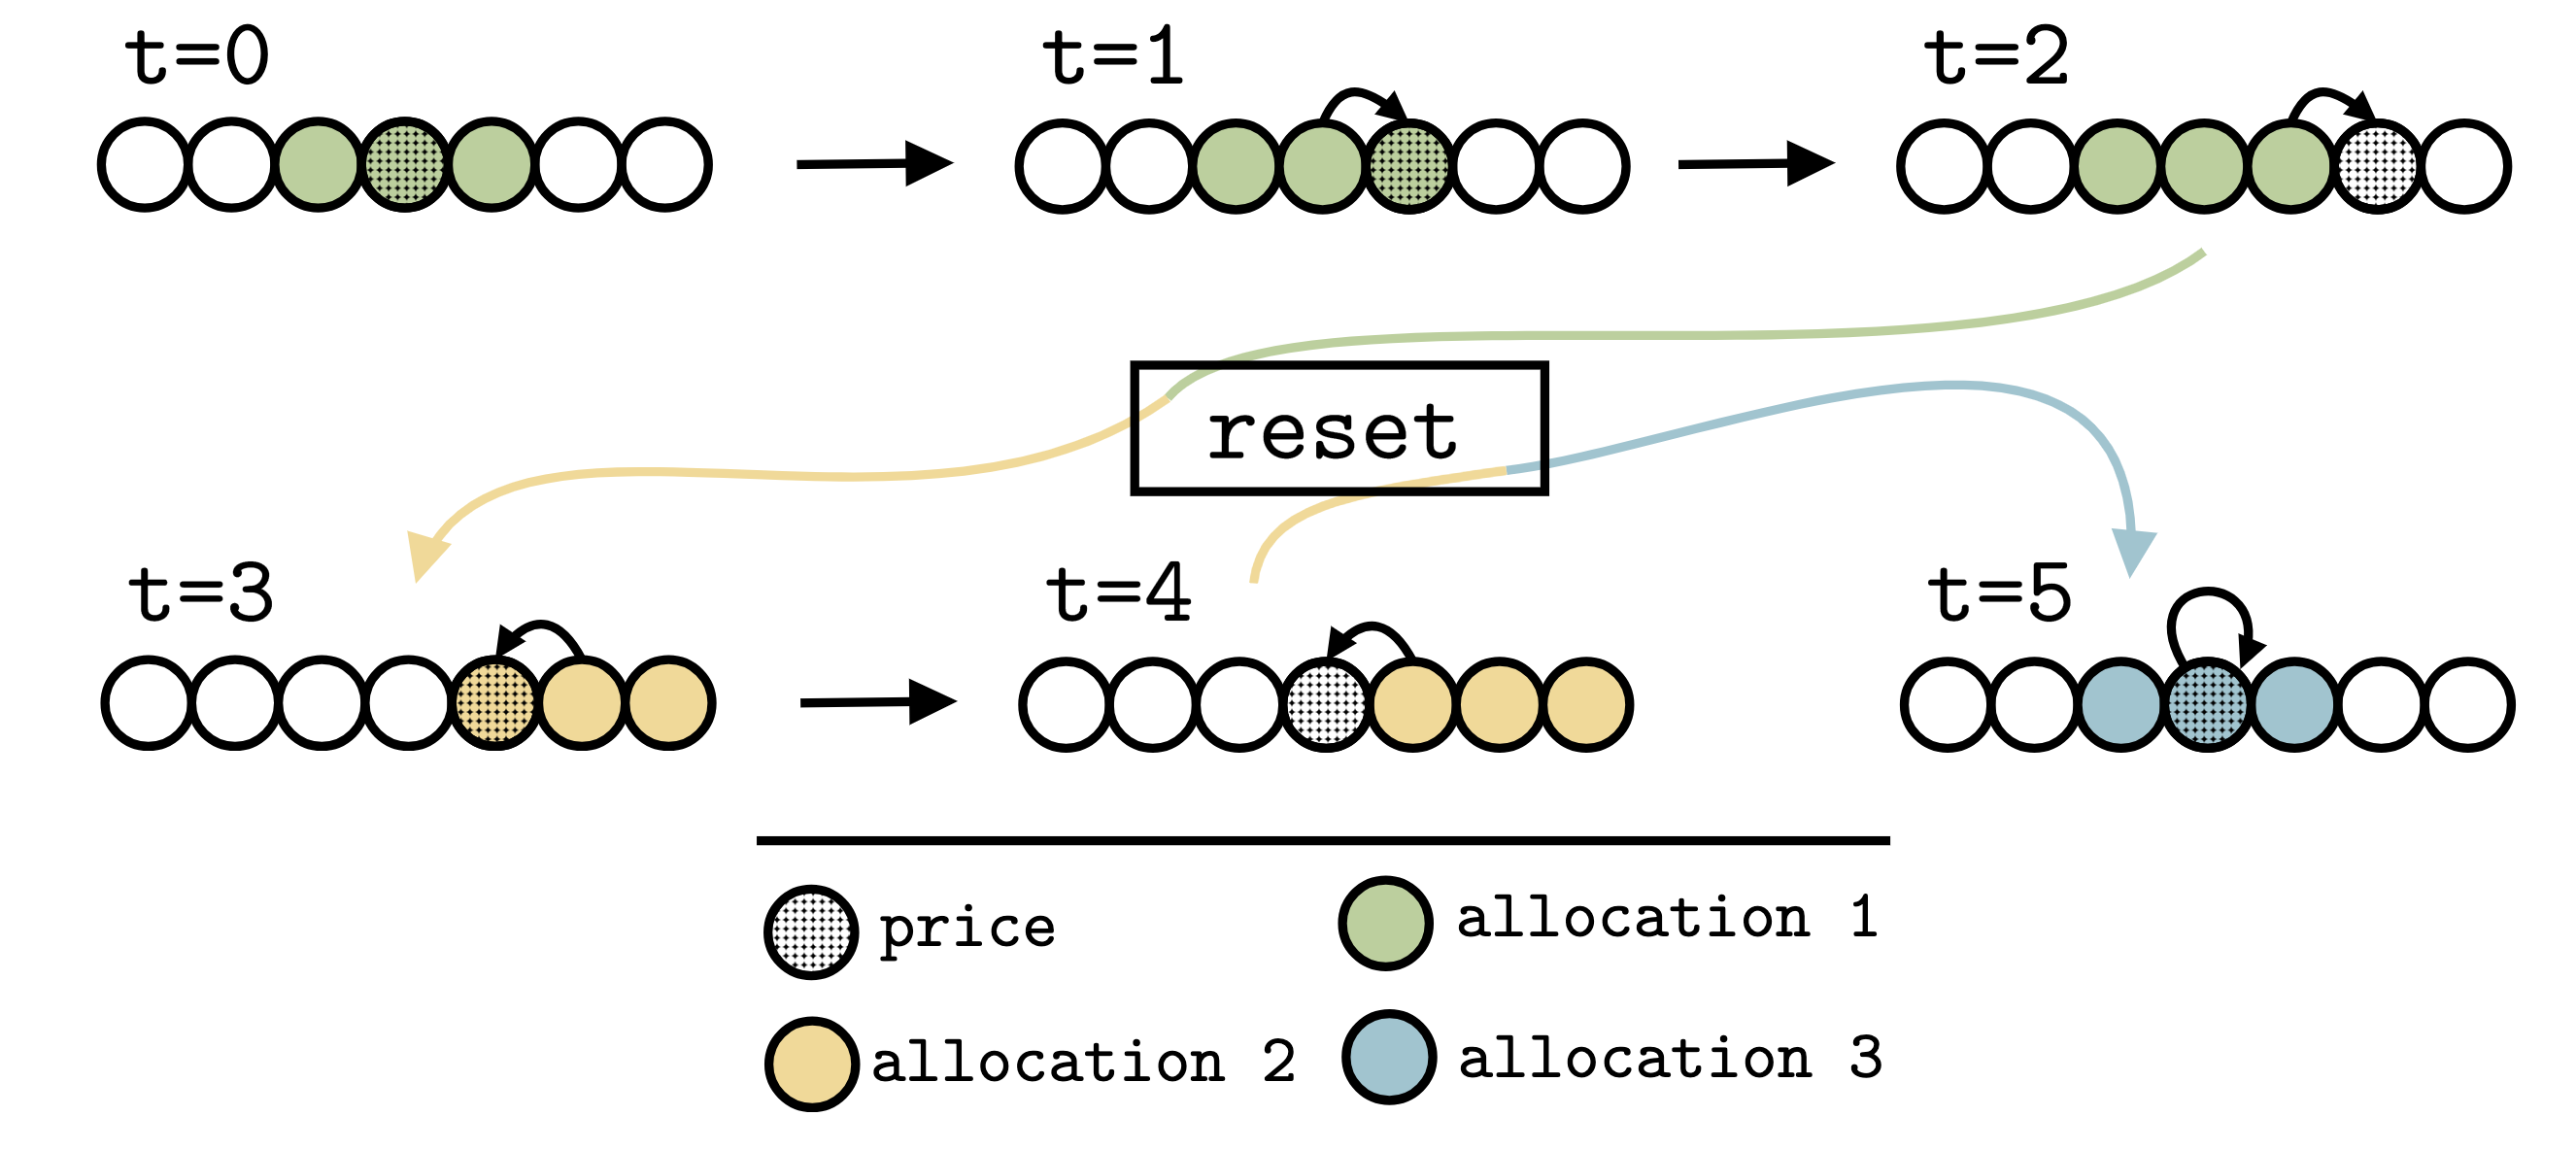
\includegraphics[width=\linewidth]{img/reset_strat.png}
    \caption{均匀的 $\tau$-重置策略,这里定义了以当前价格为中心的3个区间。每个小圆圈代表1个价格区间,黑色阴影的圆圈表示每个时间点的当前价格。
    一旦价格滑出这3个连续区间,策略 ``重置''并以重置时的价格为中心重新分配流动性。
    \label{fig:reset_strat}}
\end{figure}



% \begin{figure}
%     \centering
%     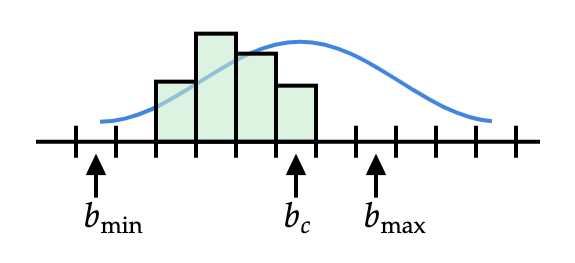
\includegraphics[width=\linewidth]{img/game.png}
%     \caption{A  liquidity provision strategy. Price movements are discretized into bins. The blue line represents the probability distribution of price movements over some amount of time, which we assume is stationary. Shown in green is the liquidity allocated to each bin ($b_c$ is current price, and $b_{\min}$ and $b_{\max}$ denote the range beyond which the provider will ``reset" its allocation). In this case, $B_{\tau}$ is the set of bins from $b_{\min}$ to (and including) $b_{\max}$.
%     \label{fig:game}}
% \end{figure}

\section{马尔可夫分析}\label{sec:markov}

\quad 在本章,我们建立了一个分析框架,来分析某种流动性重置策略的预期手续费收益效果。

%\dcp{(that said, I'm a bit worried that is not well defined when the current price gets so close to zero that the range of bins cannot be defined in the same way to the left because there aren't enough bins to the left)}

\begin{definition}\label{def:f}
用相对索引号,令 $f(i,j) \colon B_{k}\times B_{k} \to [0,1]$ 表示价格从 $B_{k}$ 内的 $i^{th}$ 区间滑动到 $B_{k}$ 内的 $j^{th}$ 区间,
\begin{align}
    f(i,j) = \mathrm{Pr}\left(P_{n+1} = b_{(j)}~|~P_n = b_{(i)}\right), \quad \text{for } i,j \in B_k.
\end{align}
注意 $f(i,j) = h(j-i)$,因为 $h$ 定义了价格滑动 $j-i$ 个区间的概率。 
\end{definition}

给定 $P_n = b_{(i)}$,下一次价格落在范围外 $b_{(j)} \notin B_{\tau}$ 的概率依然非0. 这是 $b_{(j)} \in B_{\tau}$ 的概率补集。
%
\begin{definition}
令 $g(i) \colon B_{\tau} \to [0,1]$,表示给定价格位于 $B_{\tau}$ 的第 $i^{th}$ 个区间的重置概率。
\begin{align}
    g(i) = 1 - \sum_{j \in B_{\tau}} f(i,j), \quad \text{for } i \in B_{\tau}.
\end{align}
\end{definition}
价格落在 $B_{\tau}$ 范围外,将导致流动性以 $b_s$ 为中心重新分配(根据 $\tau$-重置策略的定义),所以我们也可以将重置视同于价格落在 $b_{(0)}$ 区间。

\subsection{重置马尔科夫链}

\begin{definition}
\textit{重置马尔可夫链}, $M \in \mathbb{R}^{(2n_{\tau}+1) \times (2n_{\tau}+1)}$, 
这里 $M(i,j)$ 表示状态从当前的 $i$ 切换到状态 $j$ 的概率,描述价格在区间集 $B-{\tau}$ 中随机变化的过程,参见 $\tau$ 重置策略的定义。
于是我们有:
\[
M = 
\begin{bmatrix}
  f(-n_{\tau},-n_{\tau}) & \cdots  &f(-n_{\tau}, 0) + g(-n_{\tau}) & \cdots & f(-n_{\tau},n_{\tau}) \\
  \vdots &  & \vdots & & \vdots\\
  f(0,-n_{\tau}) & \cdots  &f(0, 0) + g(0) & \cdots & f(0,n_{\tau}) \\
  \vdots &  & \vdots & & \vdots\\
  f(n_{\tau},-n_{\tau}) & \cdots  &f\left(n_{\tau},0\right) + g(n_{\tau}) & \cdots & f(n_{\tau},n_{\tau}) \\
\end{bmatrix}.
\]
\end{definition}

\begin{definition}
给定 $B_{\tau}$, 令  $p_{\tau} \in \mathbb{R}^{1 \times (2n_{\tau}+1)}$ 表示
重置马尔可夫链的 \textit{平稳分布},这里
\begin{align}
    p_{\tau} M = p_{\tau}.
\end{align}
\end{definition}

在任何时候,给定一个 $\tau$重置策略,价格落在 $B_{\tau}$ 的第 $i^{th}$ 个区间的概率,都是 $p_{\tau}(i)$。

\subsection{流动性分配}

\quad 在执行一个 $\tau$流动性重置策略时,做市商可能希望在超出 $B_{\tau}$ 的更大范围区间上分配流动性。
%
\begin{definition}
定义一个子集 \textit{$\alpha$ bins}, $B_{\alpha} \subset B$, 表示一组以 $b_{(0)}$ 为中心的区间 $2n_{\alpha}+1$,来分配流动性。
\end{definition}

注意,
\begin{align}
    B_{\alpha} = \{b_{(-n_{\alpha})}, \cdots, b_{(0)}, \cdots, b_{(n_{\alpha})}\}.
\end{align}
与 $B_{\tau}$ 类似,我们也可以用价格区间索引号的集合来表示 $B_{\alpha}$,
\begin{align}
    B_{\alpha} = \{-n_{\alpha}, \cdots, 0, \cdots, n_{\alpha}\},
\end{align}
从上下文中可以清楚地看出用法。
%
\begin{definition}
一套 \textit{流动性分配}, $A \colon B_{\alpha} \to [0,1]$, 定义做市商分配给每个区间的流动性份额,且满足 $\sum_{i \in B_{\alpha}} A(i) \leq 1$。
\end{definition}

对于位于每一个区间 $j \in B_{\alpha}$,为了评估其分配,我们需要
(i) 任何给定时间价格落在 $b_{(j)}$ 区间的概率 (ii) 价格落在 $b_{(j)}$ 区间的效果。
%
\begin{definition}
\textit{结果矩阵}, $O \in \mathbb{R}^{(2n_{\tau}+1)\times (2n_{\alpha}+1)}$ 是,
\begin{align}
O = 
\begin{bmatrix}
  f(-n_{\tau},-n_{\alpha}) & \cdots & f(-n_{\tau}, 0) & \cdots & f(-n_{\tau},n_{\alpha}) \\
  \vdots & & \vdots &  & \vdots \\
  f(0,-n_{\alpha}) & \cdots & f(0, 0) & \cdots & f(0,n_{\alpha}) \\
  \vdots & & \vdots &  & \vdots \\
  f(n_{\tau},-n_{\alpha}) & \cdots & f(n_{\tau}, 0) & \cdots & f(n_{\tau},n_{\alpha}) \\
\end{bmatrix},
\end{align}
它代表价格从 $B_{\tau}$ 中的任何区间移动到 $B_{\alpha}$ 中的任何区间的概率。
\end{definition}
价格落在  $B_{\alpha}$ 中的第 $j^{th}$ 个区间的概率,是通过使当前区间边缘化计算得到
(取马尔可夫链平稳分布与结果矩阵每列的点乘),
%
\begin{align}
    \mathrm{Pr}\left(P_{n+1} = b_{(j)}\right) = \sum_{i \in B_{\tau}} p_{\tau}(i) \cdot f(i,j), \quad \text{for } j \in B_{\alpha}.
\end{align}

为了定义 $B_{\alpha}$ 中每个区间的效果,我们使用指数型(\textit{常绝对值风险厌恶}) 效用函数 \cite{arrow1965aspects, pratt1978risk,expectedutilityfunction}。
%
\begin{definition}\label{def:exponential_utility}
令 $u(c)$ 表示指数型效用函数,
\begin{align}\label{eq:exponential_utility}
    u(c) &= 
    \begin{cases}
    \left(1-e^{-ac}\right) / a & a\neq 0 \\
    c & a = 0,
    \end{cases}
\end{align}
这里 $a \in \mathbb{R}$ 表示绝对风险厌恶的 Arrow--Pratt 测度,用于评估做市商的风险偏好程度。

% If $a < 0$ the provider is risk-seeking, but if $a > 0$ the provider is risk-averse, and if $a=0$ the provider is risk-neutral. 
风险爱好,风险厌恶,风险中性分别对应 $a < 0$, $a > 0$, 和 $a = 0$。
\end{definition}

\begin{definition}
价格落在 $B_{\alpha}$ 的第 $j^{th}$ 个区间, 其\textit{回报}, $\reward(j)$, 与分配在该区间的流动性成正比。
令 $\kappa \in \mathbb{R}^+$ 表示比例常量,它是在下一个时间点获取到的收益,占注入流动性的比例。
根据假设 4,我们假设对于 $b_s \in B$ 的每个中心区间,在所有时间点 $t=n$ 上,$\kappa$ 都是常量。

另外,当区间滑出 $B_{\tau}$ 时,收益会导致产生 $1$ 的重置费用,因此我们有回报函数 \cite{rewardfunction}:
\begin{align}
    \reward(j) =
    \begin{cases}
        \kappa \cdot \ell \cdot A(j) & \text{for } j \in B_{\tau}, j \in B_{\alpha} \\
        \kappa \cdot \ell \cdot A(j) - 1 & \text{for } j \notin B_{\tau}, j \in B_{\alpha}. \\
    \end{cases}
\end{align}
\end{definition}

效用与做市商的风险偏好程度相关。这里,我们每次给收益增量1,定义好指数型效用函数 (公式~\ref{eq:exponential_utility}) (需要输入参数)。
这种持续的变化不会影响不同策略之间期望效用之间的对比。
%
%, we also need the utility of landing in a bin.
\begin{definition}
价格落在 $B_{\alpha}$ 中第 $j^{th}$ 区间的回报函数 $\util(j)$ 是
\begin{align}
    \util(j) = u\left(\reward(j)+1\right), \quad \text{for } j \in B_{\alpha}.
\end{align}
\end{definition}

\begin{definition}
    某个分配 $A$ 的\textit{期望效用},$E_u$,是
\begin{align}\label{eq:expected_utility}
    E_u(A) = \sum_{j \in B_{\alpha}}\mathrm{Pr}\left(P_{n+1} = b_{(j)}\right) \cdot \util(j).
\end{align}
\end{definition}

\subsection{示例}
\quad 考虑简单的下一次价格分布,
\begin{align*}
    \mathrm{Pr}(P_{n+1}= b_{(-1)}~|~P_n = b_{(0)}) &= 1/3\\
    \mathrm{Pr}(P_{n+1}= b_{(0)}~|~P_n = b_{(0)}) &= 1/3 \\
    \mathrm{Pr}(P_{n+1}= b_{(1)}~|~P_n = b_{(0)}) &= 1/3.
\end{align*}
价格滑动到下面一个区间,上面一个区间,保持不变的概率都是1/3。该价格模型在图 \ref{fig:toy_dist} 所示的马尔可夫链中表示。
\begin{figure}
    \centering
    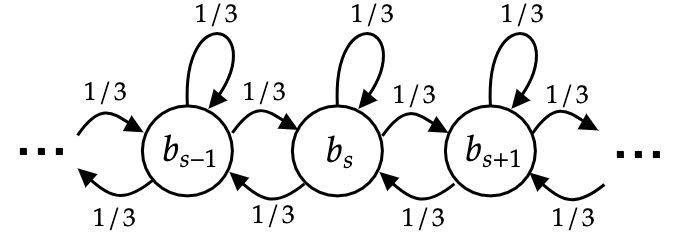
\includegraphics[width=\linewidth]{img/toy_dist.png}
    \caption{示例中的价格变化. 在每一步,都有1/3的概率向左移动,向右移动,和保持不变。
    \label{fig:toy_dist}}
\end{figure}
我们使用下面的 $\alpha$ 和 $\tau$ 区间集,
\begin{align*}
    B_\tau = B_\alpha&=\{b_{(-1)}, b_{(0)}, b_{(1)}\},
\end{align*}
这也意味着 $n_{\alpha} = n_{\tau} = 1$。现在我们可以为示例计算重置马尔可夫链,
\begin{align*}
    M = 
    \begin{bmatrix}
      1/3 & 2/3 & 0 \\
      1/3 & 1/3 & 1/3 \\
      0 & 2/3 & 1/3
    \end{bmatrix}.
\end{align*}
\begin{figure}
    \centering
    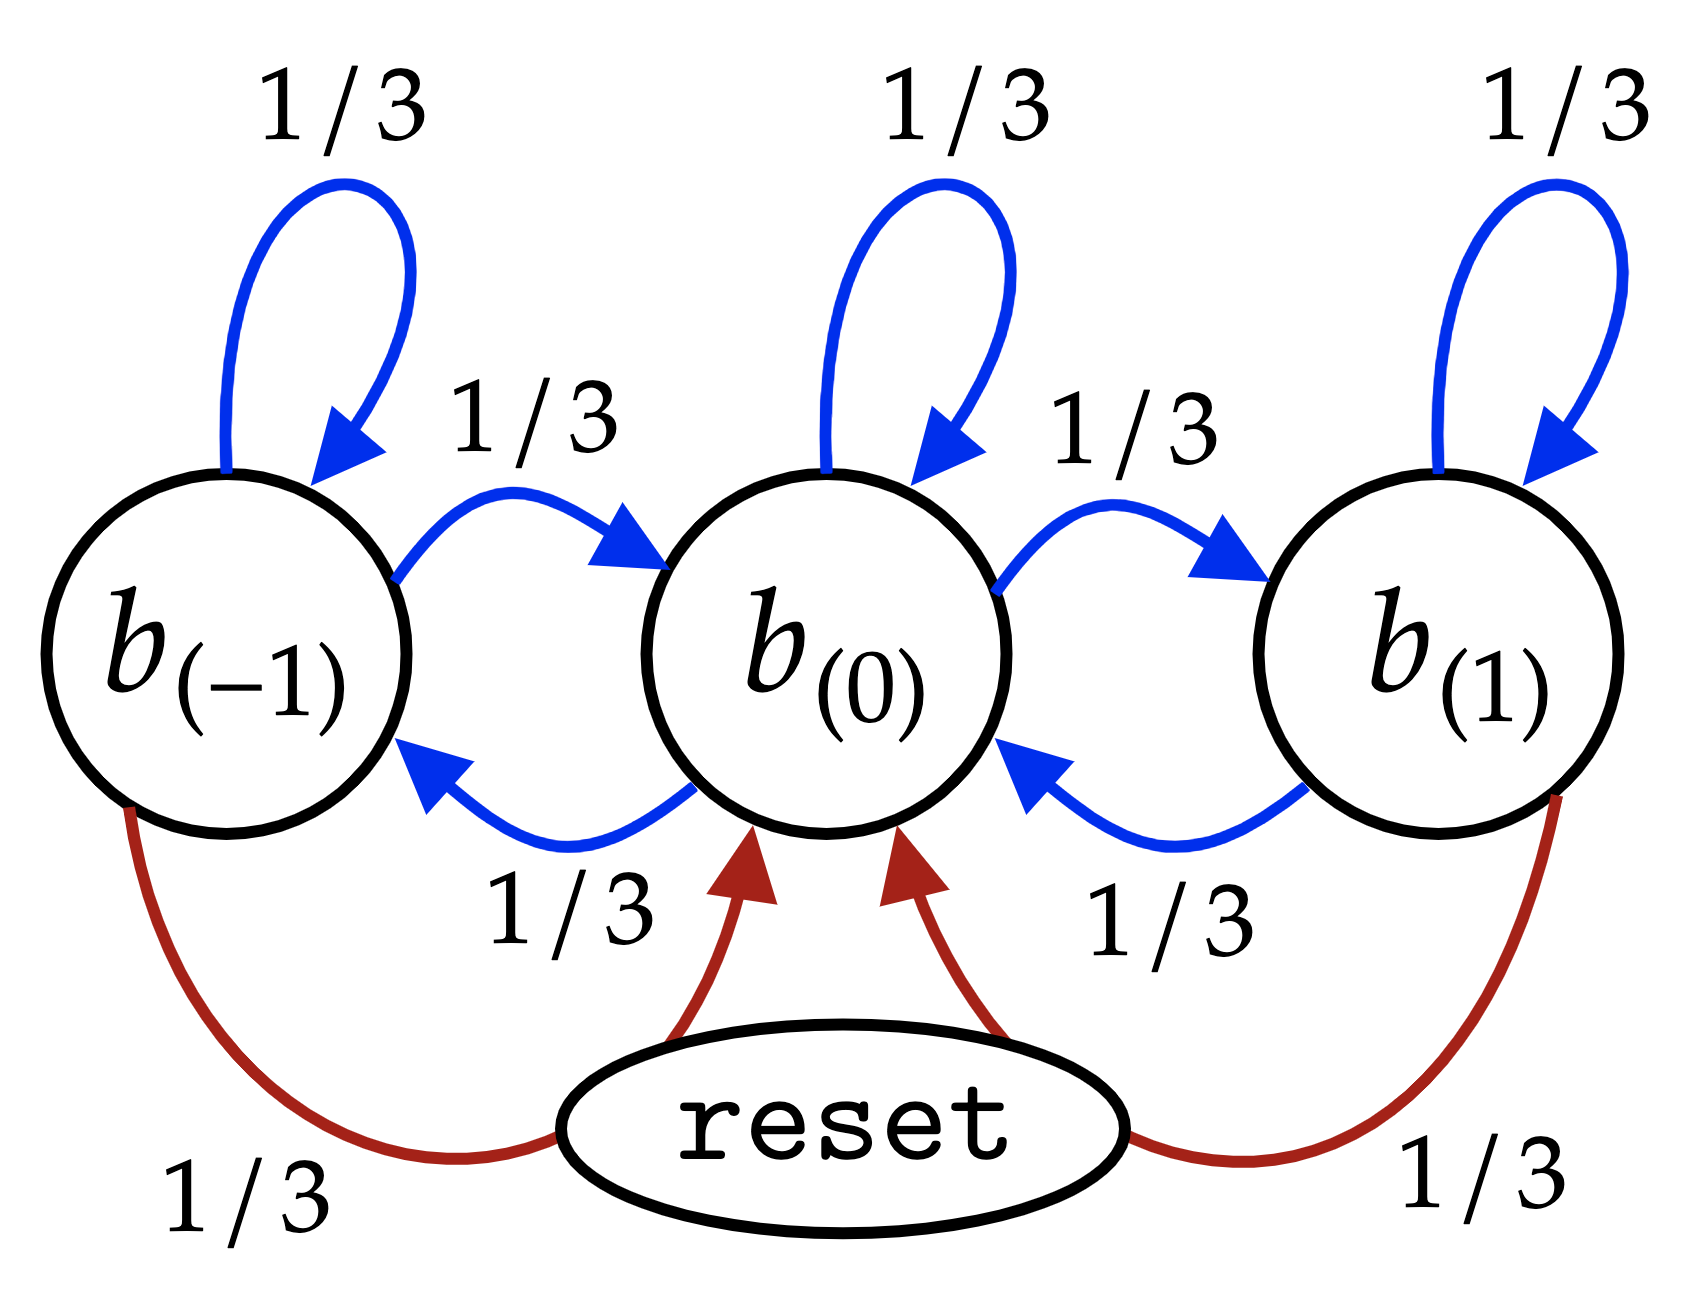
\includegraphics[width=0.7\linewidth]{img/toy_markov.png}
    \caption{示例中的重置马尔可夫链。中心节点分别有 1/3 的概率会向左,右或保持不变,那意味着它不会造成重置,且会获得一个 $+\kappa \ell /3$ 的回报。
    外部节点将以1/3的概率导致重置,从而造成 $-1$ 的负回报。
    \label{fig:toy_markov}}
\end{figure}

图~\ref{fig:toy_markov} 直观地显示了这个马尔可夫链,蓝色箭头是无需重置的滑动,红色箭头是重置滑动。
该马尔可夫链的平稳分布由特征值为1的左特征向量给出。
\begin{align*}
    p_{\tau} = 
    \begin{bmatrix}
    1/4 & 1/2 & 1/4
    \end{bmatrix}.
\end{align*}
这意味着,在任何时间步长,有一半的概率,当前价格是在策略的中间区间,有 1/4 的概率位于策略的一个边缘区间。
令分配的示例为,
\begin{align*}\label{eq:toy_allocation}
    A(j) = 1/3, \quad \textrm{for } j \in B_{\alpha},
\end{align*}
做市商在 $B_{\alpha}$ 的每个区间都分配 1/3 的流动性。我们得到结果矩阵,$O$,
\begin{align*}
    O = 
    \begin{bmatrix}
    1/3 & 1/3 & 0 \\ 
    1/3 & 1/3 & 1/3 \\ 
    0 & 1/3 & 1/3\\
    \end{bmatrix}.
\end{align*}
令 $\ell = \kappa = 1$。用平稳分布 $p_{\tau}$,和结果矩阵的每一列作点乘,我们计算出期望效用。
% \vspace{2mm}
% \begin{center}
%     \begin{tabular}{c||c|c}
%     $u$ & $u(1/3)$ & $u(0)$\\
%     \hline
%     $\mathrm{Pr}(U=u)$ & $5/6$ & $1/6$\\
%     \end{tabular}
% \end{center}
% \vspace{2mm}
如果我们令 $a=0$ (风险中性),那么,
\begin{align*}
    E_u(A) &= 1/3 \cdot 5/6 + 0 \cdot 1/6 \\
    &= 5/18 = 0.2\overline{7}.
\end{align*}
在每个时间点上,我们可以期望为提供的每单位流动性获得 $5/18$ 的回报。

% \dcp{I suggest the following }

% \begin{itemize}
%     \item Define the distribution on price changes $f(i,j)$, noting assumed stationary, also introduce the role of $n$ and $n+1$
%     \item Define $B_\tau=\{b_{s-\tau},\ldots,b_s,\ldots,b_{s+\tau}\}$, where I suggest to use $\tau$ in place of your $k$, and we note this is defined in a way that is centered on some bucket $b_s$ . Make clear that $\alpha$ corresponds to when the allocation will be ``reset"
%     \item Define the "reset-MDP", in sense of current Fig 5. 
%     \item Define the transition matrix $M$ for this reset-MDP (I don't think you need to define $M_t$ or $v_r$ explicitly, rather I think you can just define $M$ directly from $f$ and the idea of $1-\sum_j f(i,j)$ for reset probs)
%     \item Define the stationary distribution $p_\tau$ of the reset-MDP
% \end{itemize}

% \dcp{and then the following}

% \begin{itemize}
%     \item Explain that the strategy may invest in a region larger than $\tau$, and that we denote this as buckets $B_\alpha$, allowing for it to be a superset. Don't insist on this being proportional, though
%     \item State we need to compute the utility for being in each of the alpha bins, so that we can get expected utility from $p_\tau$
%     \item Introduce the  exponential utility function
%     \item Try to define utility $v_i$ for some alpha bin $i$ with as minimal notation as possible (I find the current use of $M_o$ a bit complex, and wonder if $v_i$ can be defined more directly in terms of $f$ and $p_\tau$?, without this matrix notation?). ideally the definition of $v_i$ will depend on liquidity allocation $S$, so that it is well defined for different $S$ 
%     \item Somewhere here the role of the rules of uniswap v3 should be clear 
% \end{itemize}


% \dcp{in terms of exposition, try to only use the minimal amount of notation needed, and only use matrices and vectors where helpful, and give a simple  numerical 
% illustration at the end, rather than going through these ``interludes"}

\section{流动性注入策略}\label{sec:strats}
\quad 我们现在介绍3种 $\tau$-重置策略。

\subsection{比例分配策略}\label{sub:prop-adapt}
% \dcp{this section can drop the Markov stuff, but just define the alpha-tau strategy (``proportional-adaptive") precisely. ideally we 
% just consider $\alpha\geq \tau$ and argue that $\alpha<\tau$ is not interesting}
% To demonstrate how to evaluate a liquidity provision strategy, we present a simple strategy called the $\alpha-\tau$, or proportional-adaptive, strategy. 
\quad 在该策略中,做市商按照一定的价格落在 $\alpha$ 区间的概率,按比例分配流动性。
% Let $\ell = 100$, where the units are the price of resetting a liquidity provision strategy (the associated gas fees). So the liquidity provider is allocating 100 times the cost of resetting a strategy. 
\begin{definition}
\textit{比例分配策略} 是具有以下特征的 $\tau$-重置策略:
\begin{enumerate}
    \item 区间, $b_s$, 重置策略时的价格位于此。
    \item 最小的连续区间集, $B_{\tau}$, 以 $b_s$ 为中心, 至少占下一次价格分布的概率质量中的 $\tau$。
    \item 最小的连续区间集, $B_{\alpha}$, 以 $b_s$ 为中心,至少占下一次价格分布的概率质量中的 $\alpha$。
    \item 分配函数
    \begin{align}
        A(j) \propto  h(j), \quad \text{for } j\in B_{\alpha},
    \end{align}
    根据价格落在每个区间的概率,按比例分配所有的流动性。
\end{enumerate}
\end{definition}


\begin{figure}
    \centering
    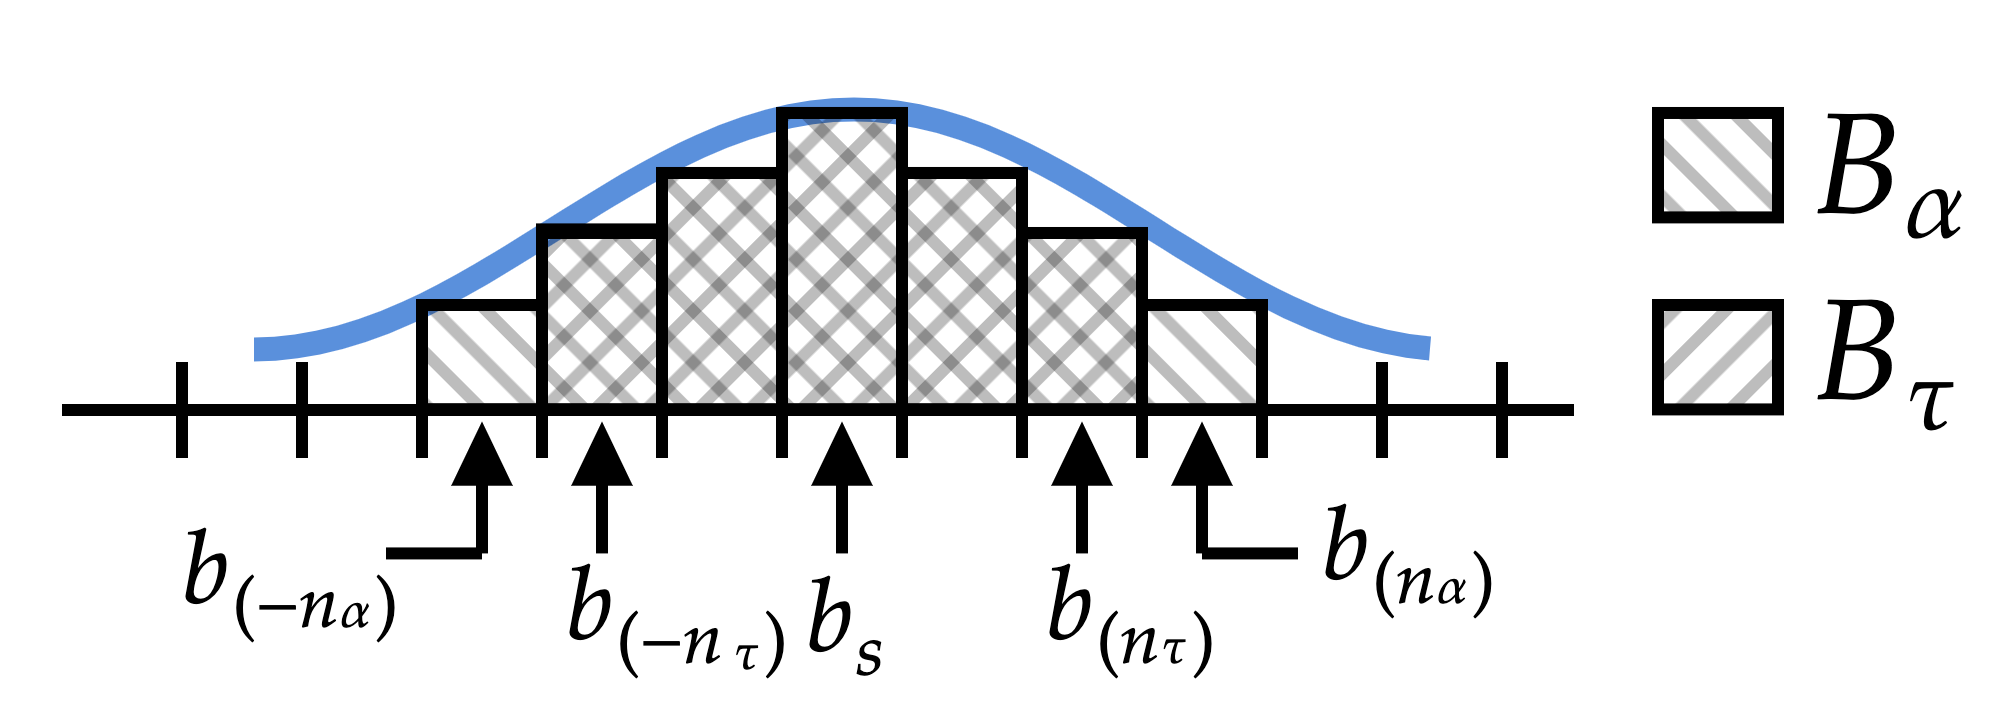
\includegraphics[width=\linewidth]{img/alpha_tau_ex.png}
    \caption{比例分配 $\tau$-重置策略的示例,这里 $\alpha > \tau$。条形图的高度表示每个区间的流动性数量。
    策略最后一次重置时,价格是 $b_s$。下一次价格概率分布用蓝色表示。``alpha" 和 ``tau" 区间集分别有图例。
    在这种情况下,中间的5个区间分别是 $B_{\alpha}$ 的一部分和 $B_{\tau}$的全部。
    \label{fig:alpha_tau_ex}}
\end{figure}
图~\ref{fig:alpha_tau_ex} 展示了比例分配策略的1个示例,对应 $\alpha > \tau$ 的情况。如果 $\alpha < \tau$,$\tau$ 区间集会比 $\alpha$ 区间集大。

\subsection{均匀分配策略}

\quad 在该策略中,做市商在一组 $\alpha$ 区间上均匀地分配流动性。
\begin{definition}
\textit{均匀分配策略} 是具有以下特征的 $\tau$-重置策略:
\begin{enumerate}
    \item 区间, $b_s$, 重置策略时的价格位于此。
    \item 一组连续价格区间集, $B_{\tau} \subset B$.
    \item 一组连续价格区间集, $B_{\alpha} \subset B$.
    \item 分配函数
    \begin{align}\label{eq:at_allocation}
        A(j) = 1 / (2n_{\alpha}+1), \quad \text{for } j\in B_{\alpha},
    \end{align}
    这里 $n_{\alpha}$ 是 $B_{\alpha}$ 中的区间数。
\end{enumerate}
\end{definition}


\subsection{最优流动性策略}
\quad 在该策略中,做市商为一组特定的连续区间集, $B_{\tau}$,在一组 $\alpha$ 区间集上最优化分配流动性 (在 $\tau$-重置策略中)。
%
\begin{definition}
\textit{最优流动性策略} 定义如下:
\begin{enumerate}
    \item 区间, $b_s$, 重置策略时的价格位于此。
    \item 一组连续价格区间集, $B_{\tau} \subset B$.
    \item 一组连续价格区间集, $B_{\alpha} \subset B$, 定义为包含从 $B_{\tau}$ 中的某个区间滑动到的每一个区间。
    % \dcp{just $B_k$ now, I think?} not quite, because B_k is the set of bins that can be transitioned to from a single bin, whereas this is from any bin in B_{\tau}
    \item 一个分配函数,$A$,就是流动性优化问题的解决方案,定义如下

\begin{equation}
    \begin{aligned}
        \max_{A \in \mathbb{R}^{B_{\alpha}}} \quad& E_u(A) = \sum_{j \in B_{\alpha}} \mathrm{Pr}\left(P_{n+1} = b_{(j)}\right) \cdot \util(j)\\
        \text{s.t.} \quad& \sum_{j \in B_{\alpha}} A(j) = 1 \\
        \quad& A(j) \geq 0 \quad \text{for } j \in B_{\alpha}.
    \end{aligned}
\end{equation}

这些约束条件规定 (i) 所有流动性都被分配,且 (ii) 分配到每个区间上的流动性皆为正。
\end{enumerate}
\end{definition}

如果存在內部解,则该优化问题允许通过拉格朗日乘子获得标准解。则该解决方案用系统表征
$$\util'(j) \cdot \mathrm{Pr}\left(P_{n+1} = b_{(j)}\right)  = \util'(k) \cdot\mathrm{Pr}\left(P_{n+1} = b_{(k)}\right) $$
对于所有的 $j, k \in B_{\alpha}$,且满足约束条件
$$\sum_{j \in B_{\alpha}} A(j) = 1$$
以及
$$A(j) \geq 0 \quad \text{for } j \in B_{\alpha}.$$

% Note that the stated solution also gives rise to a heuristic method by which to recover an interior solution: set $A(j) = 0$ for all $j \in B_{\alpha}$, and then iteratively perform gradient ascent until the budget constraint binds.

% \rithvik{should specify what set we are maximizing $A$ over. also should we put in the Lagrangian solution that characterizes the optimizer? this also gives a simple heuristic algorithm to recover the solution}

% \dcp{i'm in favor of both of these changes}

在实践中,我们使用序列最小二乘规划(SLSQP)方法 \cite{boggs1995sequential} 来解决这个约束优化问题。

\section{在以太坊历史价格数据上进行的实验}
\label{sec:results}


\begin{figure}
    \centering
    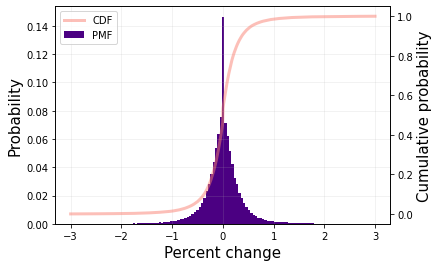
\includegraphics[width=\linewidth]{img/eth_dist.png}
    \caption{根据以太坊历史价格数据,在129个区间中下一次价格分布的百分比变化。
    \label{fig:eth_dist}}
\end{figure}

\subsection{以太坊价格数据}

\quad 为了研究前面章节所描述的流动性注入策略,我们根据以太坊历史价格数据中构建了一个下一次价格分布。
我们使用从2018年3月至2020年4月,每 10-分钟的以太坊价格数据 (100,000 个观察点)。我们计算了每一个时间点的价格变化百分比,这里
\begin{align}
    \text{percent change} = 100 \cdot (P_{n+1} - P_{n}) / P_{n}.
\end{align}
 %\rithvik{should we say something about the (lack of) sensitivity of the analysis to this assumption?}  %dcp I think it's ok not to
%
图~\ref{fig:eth_dist} 显示了下一次价格变化,在 $[-3\%,3\%]$ 范围内,每个区间变化约 $0.046\%$,共129个区间的概率分布情况。
我们使用此分布来控制价格变化的随机过程,以模拟不同流动性分配策略的回报。

% \dcp{anything to say about goodness of stability assumption?}


\subsection{比例分配策略 (风险中性做市商)}

\begin{figure*}
    \centering
    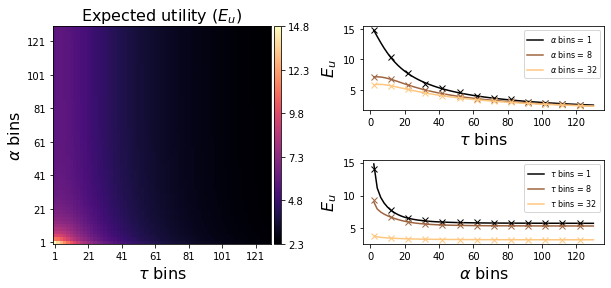
\includegraphics[width=0.8\linewidth]{img/result_sim.png}
    \caption{风险中性的做市商 ($a=0$),不同比例分配策略的期望效用。左侧:分析期望效用的密度图,不同数量的 $\tau$ 区间和 $\alpha$ 区间。
    右侧:固定 $\alpha$ 区间数,不同数量的 $\tau$ 持有区间数。实线表示分析结果,马尔可夫分析 (插入以太坊下一次价格分布)。
    $\times$ 符号表示直接模拟策略 50,000 个时间点得到的结果。
    \label{fig:result_sim}}
\end{figure*}

\quad 我们先研究一个风险中性 ($a=0$) 的做市商,使用比例分配策略,对于不同的 $\alpha$ 和 $\tau$,其效用是给定风险偏好的每个时间点的预期回报的函数。

图~\ref{fig:result_sim} (左侧) 显示预期效用的密度图,图~\ref{fig:result_sim} (右侧) 显示曲面切片,先是不同的 $n_{\alpha}$,然后是不同的 $n_{\tau}$。
我们包含两种不同的计算。实线基于分析结果 (公式~\ref{eq:expected_utility} 中插入以太坊下一次价格分布)。
$\times$ 符号表示直接模拟 50,000 个时间点的策略,得到的样本平均效用。这证实了基于马尔可夫链的分析模型的有效性。

对于一个风险中性的流动性做市商,当只有单个 $\alpha$ 和 $\tau$ 区间时,期望效用最高,即,当前区间,$b_s$。
在该策略中,做市商将所有流动性分配到单个具有最大概率的区间 (概率质量约 $0.15$)。由于在该区间分配了 $100\%$ 的流动性,对应每个时间点有 $15\%$ 的期望效用。
%, which is why the right hand plots of Figure~\ref{fig:result_sim} max out at about that value. 



% \begin{figure*}
%     \centering
%     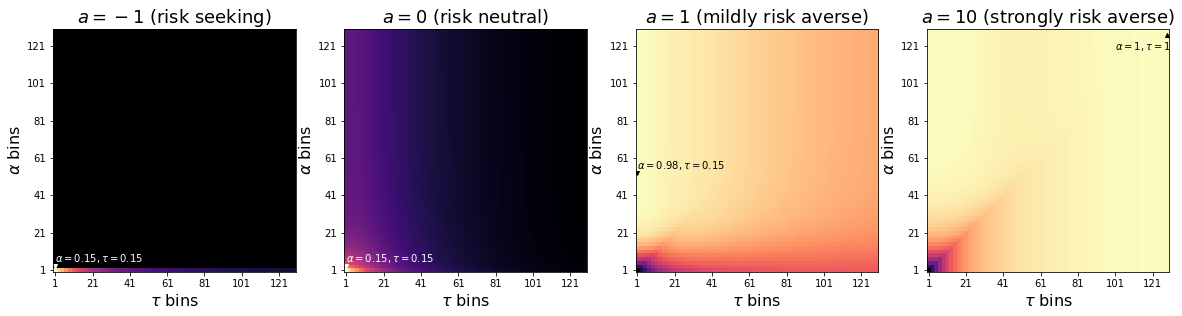
\includegraphics[width=\linewidth]{img/exponential_utility.png}
%     \caption{Expected utility for various levels of risk preference for the proportional allocation strategy. Each of the four axes plots the expected utility on a 2d grid where the $i,j$ element specifies the number of $\alpha$ and $\tau$ bins respectively. Light values are higher expected utilities, and the maximum for each plot is annotated by the text on the figure, which indicates the corresponding values of $\alpha$ and $\tau$ for that proportional strategy.}
%     \label{fig:exponential_utility}
% \end{figure*}


\subsection{最优流动性分配}


\begin{figure}
    \centering
    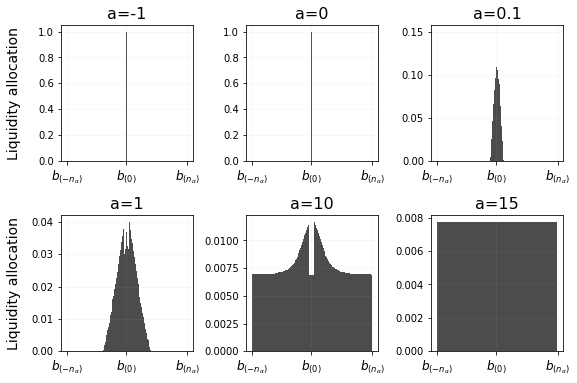
\includegraphics[width=\linewidth]{img/optimal_allocs.png}
    \caption{流动性分配最优分布的 $\tau$-重置策略,参数 $n_{\tau}$ 设为最小值,因此 $B_\tau$ 包含下一次价格分布至少 $50\%$ 的概率质量。
    图中显示了最优流动性分配的密度函数。风险爱好 ($a=-1$) 或风险中性 ($a=0$) 的做市商将所有流动性注入当前价格区间。
    当做市商变得更加风险厌恶 (例如, $a=0.1,1,10$),它倾向于用更多的区间来减小方差。
    一个极其风险厌恶的做市商 (例如,$a=15$) 在 $B_\alpha$ 区间集上使用均匀分配。
    \label{fig:optimal_allocs}}
\end{figure}


\quad 图~\ref{fig:optimal_allocs} 展示了具有不同风险偏好程度的做市商的最优流动性分配。这是参数 $n_{\tau}$ 设为最小值的 $\tau$-重置策略,因此 $B_\tau$ 包含下一次价格分布至少 $50\%$ 的概率质量。
对于风险爱好 ($a=-1$) 或风险中性 ($a=0$) 的做市商,最优分配时使用单个当前的价格区间。
这种分配会产生较高的预期回报,但相应的方差也较大。
当做市商变得更加风险厌恶 (例如, $a=0.1,1$),最优分配时使用更多的区间,同时仍然将最大比例的流动性注入具有最高概率的中心区间。
当做市商变得非常风险厌恶 (例如, $a=10$),最优分配扩展为覆盖所有的 $B_{\alpha}$ 区间,当 $a=15$ 时最优分配是在所有区间均匀分配。



\subsection{不同策略的对比}

% Figure~\ref{fig:exponential_utility} shows the expected utilities for various values of risk aversion for the proportional strategy. 

%Using the exponential utility function defined in Definition~\ref{def:exponential_utility}, we can adjust the risk preference ($a$) of a liquidity provider and see the effect on different allocations. 

\quad 图~\ref{fig:utility_comp} 对比了不同风险偏好程度下,最优,比例和均匀 $\tau$-重置策略的表现。
每种情况下,我们定义参数 $n_{\tau}$ 设为最小值,因此 $B_\tau$ 包含下一次价格分布至少 $50\%$ 的概率质量。

对于风险中性 ($a=0$) 和很低的风险厌恶 (例如,$a=0.1$),分别在 $\alpha=0.14$ 和 $\alpha=0.74$时,比例分配策略几乎是最优的。
对于风险厌恶度高 (例如,$a=10$) 的情况,均匀分布几乎是最优的。对于风险厌恶程度很高 (例如,$a=15$) 的情况,最优分配就是均匀分配。
这与图~\ref{fig:optimal_allocs}所示的最优分配是均匀的。

图~\ref{fig:opt_tau} 展示了对于不同 $\tau$ 值的最优期望效用,这里 $\tau$ 定义的是 $B_{\tau}$ 区间集包含的下一次价格分布的概率质量占比。
对于风险中性的做市商 ($a=0$),他们倾向于较小的 $\tau$ 值,因为他们愿意更频繁地调整流动性分配,并且将所有流动性注入单一的区间。
对于风险厌恶度高 (比如,$a=3$) 的做市商,他们倾向于较大的 $\tau$ 值,其结果是用大量的区间分布他们的流动性,从而降低他们所获取回报的方差。

\begin{figure}
    \centering
    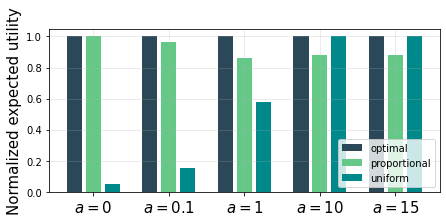
\includegraphics[width=\linewidth]{img/utility_comp.png}
    \caption{ 对不同风险偏好程度的最佳比例和均匀分配,及最优策略的期望效用 (不同 $a$ 值)。
    对每个 $a$ 值,效用由该 $a$ 值的期望最佳效用给出标准。对于风险偏好度偏高 (例如, $a=0,0.1,1$) 的做市商,比例分配策略明显优于均匀分配策略。
    对于强烈风险厌恶的做市商 (例如, $a=10,15$),均匀分配策略是最优的。
    \label{fig:utility_comp}}
\end{figure}

\begin{figure}
    \centering
    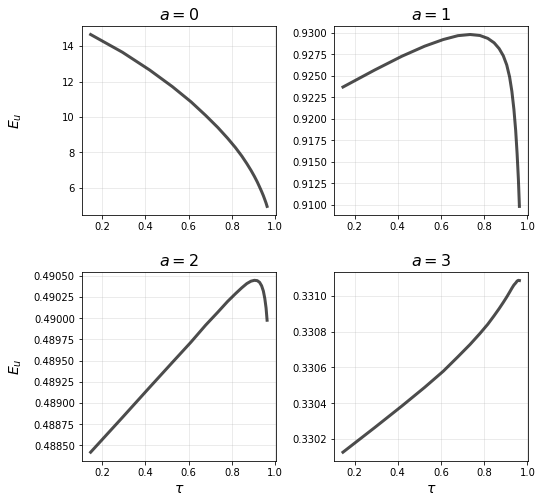
\includegraphics[width=\linewidth]{img/opt_tau.png}
    \caption{ 作为 $\tau$ 值的函数,最优 $\tau$-重置策略的期望效用。
    这里,我们将 $\tau$ 视作价格落在 $B_\tau$ 区间内的概率质量。 风险中性 ($a=0$) 的做市商倾向于小的 $\tau$ 值,
    愿意迅速调整他的流动性分配。对于一个更加风险厌恶的做市商 (例如, $a=3$),则相反。由于他们在更多的区间分配流动性,
    最优 $\tau$ 值应该尽可能高,以覆盖更多的价格区间,并进一步减小回报的方差。
    \label{fig:opt_tau}}
\end{figure}

\subsection{与 Uniswap v2 的对比}

\quad 根据以太坊的历史价格数据,我们可以对流动性注入策略的表现进行回归测试,并与 Uniswap v2 流动性注入作对比。
回想一下,在 Uniswap v2 中,做市商在注入流动性时无法指定价格区间。

图~\ref{fig:eth_price} 展示了我们用于测试的时间段中以太坊的历史价格。
如插图所示,黑线代表当时以太坊的价格,红线和蓝线分别代表对应下一次价格分布的 $\tau-0.5$,$a=0.1$ (图~\ref{fig:optimal_allocs} 右上的分配方式)的情况下, 
最优 $\tau$-重置策略的  $\alpha$ 和 $\tau$ 区间边界。 
这展示了该策略如何重新以当前价格为中心,定期调整注入的流动性。

为了模拟 Uniswap v2 的流动性注入策略,我们在该数据的整个价格范围内均匀地进行分配。
在这个例子中,价格范围从 81 USD 到 830 USD,我们根据下一次价格分布的经验计算得到的间隔,将该价格范围离散化为约 5,500 个区间 (图~\ref{fig:eth_dist})。

我们在这 5,500 个区间均匀分配流动性,可以在每个时间点上提供 $u(1/5500, a)$ 的保证效用。
我们通过找到最优 $\tau$-重置策略,并相应地分配流动性来计算数据集中每个价格的效用,将其与 v3 作对比。
对于略有风险厌恶 $(a=0.1)$ 的做市商,最优 $\tau$-重置策略比 v2 策略效用提升 $230$ 倍。

\begin{figure*}
    \centering
    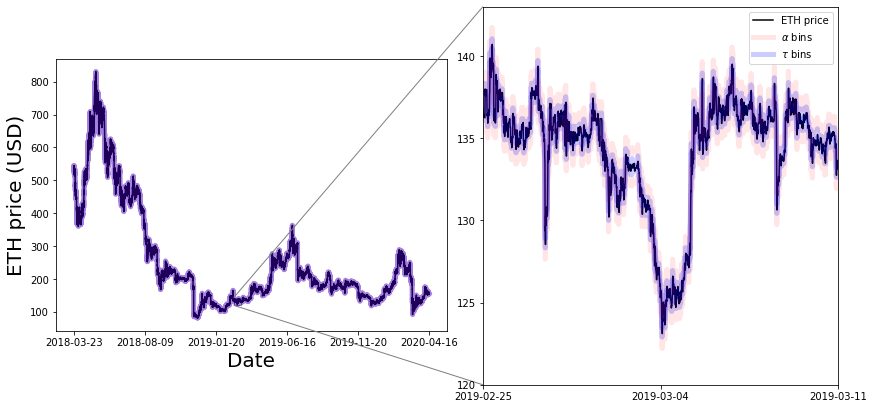
\includegraphics[width=0.7\linewidth]{img/eth_price.png}
    \caption{ 对于 $\tau=0.5$, 用以太坊历史价格数据回测最优 $\tau$-重置策略。
    红线表示每个时间点的 $\alpha$ 区间的宽度,蓝线表示 $\tau$ 区间的宽度。
    使用该策略,比在整个价格范围均匀地注入流动性 (Uniswap v2 分配),做市商获得超过 230 倍的回报。 
    \label{fig:eth_price}}
\end{figure*}

% \begin{figure}
%     \centering
%     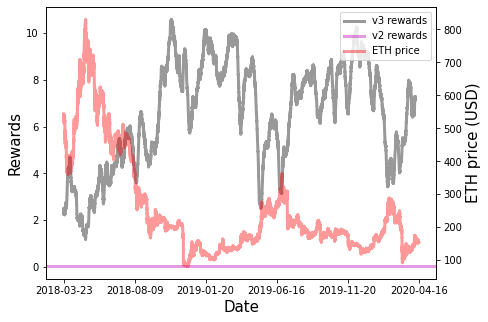
\includegraphics[width=\linewidth]{img/rewards_price.png}
%     \caption{Rewards backtest.}
%     \label{fig:rewards_price}
% \end{figure}

% \blindtext
% \blindtext
% \blindtext
% \blindtext
% \blindtext

\section{结论}\label{sec:conclusion}
\quad 本项工作探讨了 Uniswap v3 协议带来的流动性注入策略问题。
我们介绍了广泛的 $\tau$-重置策略,并概述了一种用户分析计算它们的期望效用的技术。
我们描述了该策略的3种不同实现,并在以太坊历史价格数据上构建了下一次价格分布,对比了3种策略的表现。
给定 $\tau$ 区间的选择,和下一次价格分布,我们可以找到最优 $\tau$-重置策略。
我们发现最优 $\tau$-重置策略的期望效用是 v2 策略效用的 200 倍以上。

%\subsection{Future work}\label{sec:future}

%As the TVL and trading volume on v3 grow, we expect to see many new strategies emerge. 
%
我们希望这项工作可以作为正式化和比较这些策略性能的第一步。
本框架仅代表完整策略集的一个子集,考虑使用相同方法在更广泛的时间段进行流动性分配,执行以当前价格为中心的策略,并由足够大的价格变动触发重新分配。
更丰富的策略类别,还可以根据最近的价格变动趋势,修改流动性分配和重置策略。

在多个做市商背景下,研究流动性注入问题将是有趣的。
在本文中,我们研究了单个 v3 玩家与一组 v2 玩家之间的投资对比。在未来的工作中,我们看到了研究 Uniswap v3 流动性注入设置的紧急均衡特性的机会。
在 Uniswap v3 上进行策略的实证研究也很有趣。
另外,Uniswap v3 和 gas 价格之间存在着有趣的宏观层面的关联。
如果 gas 费用低,流动性做市商就会更频繁地调整他们的头寸,那又可能导致 gas 费上升。
理解 Uniswap 和 gas 价格之间由此产生的动态效应和关联,是另一个有希望的方向。

%% The acknowledgments section is defined using the "acks" environment
%% (and NOT an unnumbered section). This ensures the proper
%% identification of the section in the article metadata, and the
%% consistent spelling of the heading.
\begin{acks}
这项工作部分得到了哈佛大学计算与社会研究中心的两份慷慨礼物的支持,二者都支持应用密码学和社会学的研究。 
\end{acks}

%%
%% The next two lines define the bibliography style to be used, and
%% the bibliography file.
\bibliographystyle{ACM-Reference-Format}
\bibliography{refs}

\end{document}
\endinput
